\documentclass[11pt,a4paper]{article}

\usepackage[T1]{fontenc}
\usepackage{lmodern}
\usepackage{microtype}
\usepackage{amsmath,amssymb,amsthm}
\usepackage{mathpartir}
\usepackage{stmaryrd}
\usepackage{booktabs}
\usepackage{tabularx}
\usepackage{graphicx}
\usepackage{listings}
\usepackage{xcolor}
\usepackage[margin=2.5cm]{geometry}
\usepackage{enumitem}
\usepackage[font=small,labelfont=bf]{caption}
\usepackage{xurl}
\usepackage[hidelinks]{hyperref}

\newtheorem{theorem}{Theorem}
\newtheorem{lemma}{Lemma}

\definecolor{kw}{HTML}{1F4E79}
\definecolor{cm}{HTML}{5A6B5A}
\definecolor{st}{HTML}{8B3A0E}

\lstdefinelanguage{NucleScript}{
  morekeywords={pool,let,fn,returns,store,into,retrieve,delete,from,confirm,
    hardware,physical_key,simulate,under,pipeline,encode,using,protect,with,
    redundancy,verify,roundtrip,match,if,else,for,in,decode,reads,against,
    blind,expect,recovery,retain,storage,codec,profile,coverage,enum,test,assert},
  morecomment=[l]{//},
  morestring=[b]",
  sensitive=true
}
\lstset{
  language=NucleScript,
  basicstyle=\ttfamily\small,
  keywordstyle=\color{kw}\bfseries,
  commentstyle=\color{cm}\itshape,
  stringstyle=\color{st},
  columns=fullflexible,
  keepspaces=true,
  breaklines=true,
  breakindent=2em,
  frame=lines,
  framesep=4pt,
  xleftmargin=6pt,
  xrightmargin=6pt,
  aboveskip=8pt,
  belowskip=8pt,
  captionpos=b
}

\newcommand{\Syn}{\mathsf{Syn}}
\newcommand{\Seq}{\mathsf{Seq}}
\newcommand{\Des}{\mathsf{Des}}
\newcommand{\allowed}{\mathit{allowed}}
\newcommand{\known}{\mathsf{known}}
\newcommand{\param}{\mathsf{param}}
\newcommand{\fits}{\mathit{fits}}
\newcommand{\opq}{\mathit{opq}}
\newcommand{\clo}{\mathsf{clo}}
\newcommand{\app}{\mathbin{+\!\!+}}
\newcommand{\nsl}[1]{\texttt{#1}}

\title{NucleScript: Effects, Confirmations and Channel-Typed Pools\\
for DNA Data Storage Programs}
\author{Vyom Kulshrestha\\
\small Independent Researcher, India\\
\small ORCID \href{https://orcid.org/0009-0009-1434-7148}{0009-0009-1434-7148}}
\date{Technical report, 8 November 2026\\
\small NucleScript 1.0, NucleOS v0.1.70\\
\small \href{https://doi.org/10.5281/zenodo.24057685}{doi:10.5281/zenodo.24057685}}

\begin{document}
\maketitle

\begin{abstract}
Storing data in DNA means paying for synthesis and sequencing, destroying
material when data is deleted, and reading it back through noisy channels
whose error rates depend on the instrument. NucleScript is a small
language for writing such storage programs. A pool's type names the
sequencer profile it was read through and an error rate that consensus
lowers. Operations that synthesise, sequence or delete have effects, each
needs a confirmation written at the operation, and a function type can
bound the effects of the closures passed through it. NucleScript is
implemented in Rust as part of NucleOS, which supplies the codecs
(ternary, DNA Fountain, Yin-Yang, HEDGES), Reed--Solomon parity, a noise
simulator with channels measured from real oligo pools, and consensus and
clustering of real reads. The checker is checked in two ways. A runtime
monitor runs the shipped examples and generated programs and compares
what each did with what the checker promised; with the work of writing the
rules down formally, it has found eight defects, all fixed. A Lean~4
proof shows, for a core calculus with closures, aliases, closures the
checker cannot see into, and higher-order functions, that an accepted
program performs only confirmed operations, only effects the checker
reports, and nothing a closure's ceiling forbids. On public data, a
NucleScript program decodes 99.73\% and 96.94\% of the strands of two
Illumina oligo pools with their labels, and 99.73\% and 95.82\% without
them; the same decoder recovers 94.7\% of 2,000 MinION clusters. No
NucleScript program has yet driven a real synthesis or sequencing run.
\end{abstract}

\section{Introduction}

DNA data storage writes a file by synthesising short oligonucleotides
that encode it, and reads the file back by sequencing them
\cite{church2012,goldman2013,erlich2017,organick2018}. Each write costs
money and laboratory time. Each read costs more and returns many noisy,
unordered copies of each strand, so a decoder has to cluster them, take a
consensus, and fill the gaps with an outer code. Deleting data means
destroying physical material. The channel is very different across
instruments: Illumina reads miss about one base in a thousand, while
nanopore reads get several percent wrong.

The software around this is a set of libraries and simulators
\cite{chamaeleo,mesa,storalator,dnatoolkit}, driven by scripts. Nothing
checks such a script before it runs. A script can delete a pool's
contents without anyone confirming it, store data at a redundancy that
the chosen sequencer cannot recover from, or ask for a retention period
the storage medium cannot reach. In ordinary programs such mistakes cost
a rerun. Here they cost a synthesis order or a pool of molecules.

NucleScript makes these properties part of a program's types. This
report describes the language and its implementation, and then asks how
far its checker can be trusted. Its contributions are:

\begin{itemize}[leftmargin=*,itemsep=2pt]
\item A language design (Sections~\ref{sec:lang} and~\ref{sec:types}):
  pools typed by the channel they were read through, effects for
  synthesis, sequencing and deletion whose confirmations are written at
  the operation and checked at compile time, and effect ceilings on
  function types that bound what a closure passed through them may do.
\item An implementation inside NucleOS (Section~\ref{sec:impl}), with
  four codecs, Reed--Solomon parity, channels measured from real oligo
  pools, decoding of real reads, an editor extension and a stability
  promise for language version~1.0.
\item A runtime monitor and a random program generator that check the
  checker's promises on running programs (Section~\ref{sec:monitor}).
  Together with formalising the rules, they found eight defects in the
  checker, all now fixed.
\item A proof in Lean~4 \cite{lean4} that the effect and confirmation
  rules keep three of the checker's four promises for a core calculus of
  the language (Section~\ref{sec:proof}).
\item An evaluation of decoding on public sequencing data
  (Section~\ref{sec:eval}): a MinION dataset and two Illumina oligo pools,
  the latter decoded from inside a NucleScript program.
\end{itemize}

The limits come first: no NucleScript program has driven a real
synthesizer or sequencer, and the decoding results use datasets other
groups produced. Section~\ref{sec:limits} lists the rest.

\section{Background}
\label{sec:background}

\paragraph{Writing.} Oligo pools are synthesised in parallel on arrays,
typically 100 to 350 nucleotides per strand. Synthesis is cheaper and
more accurate when the GC content stays near half and runs of one base
(homopolymers) are short. It introduces substitutions, insertions and
deletions, and some strands are lost altogether. A codec maps bits to
bases while respecting these constraints: the rotating ternary code of
Goldman et al.~\cite{goldman2013}, DNA Fountain's screened LT code
\cite{erlich2017}, the Yin-Yang code \cite{yinyang}, and HEDGES
\cite{hedges}, which corrects insertions and deletions directly.

\paragraph{Reading.} A sequencer returns reads in no particular order,
several per strand. Coverage varies from strand to strand, roughly
log-normally, and some strands get no reads. Illumina reads have mostly
substitutions; nanopore reads have substitutions, insertions and
deletions at a few percent each. Decoding clusters the reads by strand
\cite{rashtchian2017}, takes a consensus per cluster
\cite{trellisbma}, and lets an outer erasure code such as Reed--Solomon
fill in strands that are missing or wrong.

\paragraph{Keeping.} DNA decays. Strand breaks follow Arrhenius kinetics,
measured for DNA in bone \cite{allentoft2012}, in silica
\cite{grass2015} and in dry anoxic capsules \cite{coudy2021}, so whether
a file is still readable after a given time depends on the medium, the
temperature and the strand length.

\section{The language by example}
\label{sec:lang}

A NucleScript program declares pools and runs operations on them.
Listing~\ref{lst:hero} declares a pool written with the Yin-Yang codec at
4$\times$ redundancy and read on Illumina.

\begin{lstlisting}[caption={A pool, a simulated read, a consensus and a pipeline (\texttt{hero.nsl}).},label=lst:hero]
pool medical_archive: DnaPool {
    codec: YinYang,
    redundancy: 4x,
    profile: Illumina
}

let noisy: Pool<Illumina, 0.35%> = simulate medical_archive under Illumina
let recovered: Pool<Recovered> = consensus_vote(noisy, coverage: 10x)

pipeline archive_patient_records {
    encode "patient_records_2026.csv" using YinYang,
    protect with redundancy 4x,
    store into medical_archive,
    verify roundtrip
}
\end{lstlisting}

The pool declaration is checked at compile time against the constraints
of Section~\ref{sec:background}. The type \nsl{Pool<Illumina, 0.35\%>}
says the simulated read went through the Illumina profile and carries
its error rate; \nsl{consensus\_vote} at 10$\times$ coverage gives a
recovered pool with a lower rate. The pipeline encodes a real file,
adds parity strands, stores them in the simulated pool, and
\nsl{verify roundtrip} decodes the file back and compares it byte for
byte.

\paragraph{Effects and confirmations.} Storing, synthesising, sequencing
and deleting have effects. A delete needs \nsl{confirm physical\_key}
written on the same statement, and \nsl{synthesise} and \nsl{sequence}
need \nsl{confirm hardware}. Wrapping an operation in a function does not
hide it:

\begin{lstlisting}[caption={A delete inside a function, without its confirmation.},label=lst:purge]
fn purge() returns Void {
    delete "old_archive.bin" from archive
}
let result: Void = purge()
\end{lstlisting}

The checker rejects Listing~\ref{lst:purge} twice, once at the delete and
once at the call, which is Destructive because the function is. Adding
the confirmation to the delete, where the effect originates, fixes both.
\nsl{nucle explain} prints each top-level declaration's effect before
anything runs.

\paragraph{Effect ceilings.} Higher-order functions take closures. A
parameter's type can carry a ceiling, and every closure bound into that
slot must fit it:

\begin{lstlisting}[caption={A closure parameter with a ceiling (\texttt{effect\_annotated\_closure.nsl}, shortened).},label=lst:ceiling]
fn archive_with_cleanup_policy(cleanup: Fn() -> Void confirm physical_key) returns Void {
    let x: Void = cleanup()
}

fn run_cleanup() returns Void {
    let purge_expired: Fn() -> Void confirm physical_key = fn() -> Void {
        delete "sample_a.txt" from archive confirm physical_key
    }
    let result: Void = archive_with_cleanup_policy(purge_expired)
}
\end{lstlisting}

Inside \nsl{archive\_with\_cleanup\_policy}, the call \nsl{cleanup()} is
trusted to be Destructive and confirmed without seeing the closure,
because each closure that can reach the parameter was checked where it
was bound. A closure that stored as well as deleted would be rejected
there.

\paragraph{Results, retention and real reads.} Operations that can fail
at run time return \nsl{Result}, which \nsl{?} and \nsl{match} take
apart. Listing~\ref{lst:retain} asks for ten thousand years of
readability, which a pool kept in bone at 25\,$^\circ$C cannot give, and
falls back to an encapsulated pool at $-20$\,$^\circ$C. The check runs
against the strands actually written, using the published decay
kinetics of the pool's storage medium.

\begin{lstlisting}[caption={A retention requirement with a fallback (\texttt{retention\_policy.nsl}, shortened).},label=lst:retain]
pool shelf: DnaPool { codec: Ternary, redundancy: 3x, profile: Twist, storage: bone at 25C }
pool capsule: DnaPool { codec: YinYang, redundancy: 3x, profile: Twist, storage: encapsulated at -20C }

fn archive_for(target: File) returns Result<DnaFile, Str> {
    let attempt: Result<DnaFile, Str> = store target into shelf { retain: 10000y }
    let saved: DnaFile = match attempt {
        Ok(file) => file,
        Err(reason) => (store target into capsule { retain: 10000y })?
    }
}
\end{lstlisting}

Finally, \nsl{decode reads} takes real sequencing reads and the designed
references, decodes them with and without the dataset's cluster labels,
and stops the program if recovery falls short:

\begin{lstlisting}[caption={Decoding real MinION reads (\texttt{real\_reads.nsl}, with paths from the repository root).},label=lst:reads]
decode reads "nucle_ecc/tests/fixtures/cnr/Clusters.txt"
    against "nucle_ecc/tests/fixtures/cnr/Centers.txt" {
    blind,
    expect recovery > 90%
}
\end{lstlisting}

The language also has functions generic over a pool's profile
(\nsl{fn recover\_from<P>(source: Pool<P, 0.35\%>)}), user enums with
exhaustive matching, package imports, \nsl{test} blocks with
\nsl{assert}, and compile-time \nsl{if} and \nsl{for}.

\section{Types and effects}
\label{sec:types}

\subsection{Pools typed by their channel}

A pool's type is \nsl{Pool<}$P$\nsl{, }$r$\nsl{>}, where $P$ is a
sequencer profile or \nsl{Recovered}, and $r$ an error rate in percent.
Simulating a pool under profile $P$ gives the profile's default rate
(0.35\% for Illumina, 5\% for Nanopore, 0.03\% for Twist and 0.05\% for
IDT). \nsl{consensus\_vote} at coverage $c \ge 2$ divides the rate by
$c^2$, a deliberately simple model of majority voting that the type
system treats as a bound, not a prediction. Where branches produce pools,
as in the arms of a \nsl{match}, the result takes the worse rate: the
type promises only the noise every branch can guarantee. A declared rate
that disagrees with the inferred one is an error.

Functions can be generic over the profile. A generic body is checked
again for each profile it is called with, so a warning that applies only
to Nanopore fires at a Nanopore call and not an Illumina one. A recovery
expectation such as \nsl{expect recovery > 99.9\%} is checked against the
profile and coverage, and the optimizer raises redundancy that is too low
for the chosen profile before anything is stored.

\subsection{Effects}

An operation may have three effects: Synthesis ($\Syn$), Sequencing
($\Seq$) and Destructive ($\Des$). \nsl{nucle explain} reports the worst
of a declaration's effects in the order
$\mathsf{Pure} < \Seq < \Syn < \Des$. The checker keeps the whole set,
because ceilings need it. Table~\ref{tab:rules} gives the rules. $\Gamma$
holds the program's functions, the closures \nsl{let}-bound so far in the
enclosing blocks, and the ceilings of annotated \nsl{Fn} parameters.

\begin{table}[t]
\centering
\small
\begin{tabularx}{\linewidth}{@{}lX@{}}
\toprule
Form & Effects \\
\midrule
\nsl{store f into p} & $\{\Syn\}$ \\
\nsl{simulate store}, \nsl{retrieve}, \nsl{decode reads}, declarations & $\emptyset$ \\
\nsl{delete f from p} & $\{\Des\}$ \\
\nsl{synthesise ...}, \nsl{sequence ...} & $\{\Syn\}$, $\{\Seq\}$ \\
a pipeline with a \nsl{store into} step & $\{\Syn\}$ \\
a closure literal & $\emptyset$: defining one runs nothing \\
$f(a_1,\dots,a_n)$, $f$ a function or closure in $\Gamma$ & $E(\text{body of } f) \cup E(a_i)$ for each closure $a_i$ passed to an unannotated \nsl{Fn} parameter \\
$p()$, $p$ typed \nsl{Fn(...) -> T confirm hardware} & $\{\Syn\}$ \\
$p()$, $p$ typed \nsl{Fn(...) -> T confirm physical\_key} & $\{\Des\}$ \\
$p()$, $p$ an unannotated \nsl{Fn} parameter & $\emptyset$; the call that passed the closure adds its effects \\
$g()$, $g$ a closure the checker cannot trace & every effect \\
\nsl{match}, \nsl{if} & the union over every arm or branch, taken or not \\
a block $d_1 \dots d_n$ & $\bigcup_i E(d_i)$, with \nsl{let} bindings of closures, aliases and annotated types entering $\Gamma$ \\
\bottomrule
\end{tabularx}
\caption{Effect rules. A recursive call contributes $\emptyset$ to its own
strongly connected component, which gives the least fixed point: a
recursive function that deletes is still Destructive.}
\label{tab:rules}
\end{table}

\paragraph{Confirmation.} Every operation that needs a confirmation
carries it on its own statement. A call is confirmed when every operation
its effects come from is. A \nsl{store} needs no confirmation; the
checker warns about stores that are not simulated.

\paragraph{Ceilings.} Binding a closure $c$ into a slot with ceiling $k$,
by passing it to an annotated parameter or \nsl{let}-binding it with an
annotated type, requires $E(c) \subseteq \allowed(k)$ and requires every
operation in $c$ to be confirmed. Here
$\allowed(\nsl{hardware}) = \{\Syn, \Seq\}$ and
$\allowed(\nsl{physical\_key}) = \{\Des\}$. Comparing the whole set matters: a closure that
stores and deletes has worst effect Destructive, which fits
\nsl{confirm physical\_key}, but its store does not.

\paragraph{Closures the checker cannot see into.} A closure returned by a
function, or taken out of an enum, is a value whose body the effect walk
never meets. A call through one has every effect, so it fits no ceiling
unless the \nsl{Fn} type it comes through declares one, which the checker
enforced where the closure was created.

\paragraph{Parameters without a ceiling.} Inside its function, a call
through an unannotated \nsl{Fn} parameter counts as $\emptyset$, because
each call site adds the effects of the closure it passes. That is right
for reporting and wrong under a ceiling: a function that passes such a
parameter on to a \nsl{confirm hardware} slot runs whatever closure its
own caller chose under that ceiling. So where a ceiling is checked, a
call through an unannotated parameter has every effect.

\section{Implementation}
\label{sec:impl}

NucleScript is implemented in the NucleOS workspace: 14 Rust crates and
about 54,000 lines of Rust, of which the compiler crate \nsl{nucle\_lang}
is about 17,000. A program goes through a lexer and parser, a type and
effect checker that also resolves compile-time \nsl{if} and \nsl{for}, a
mid-level representation, an optimizer that raises redundancy for the
chosen profile and coverage, and either a simulation backend or an
interpreter that runs the operations against the NucleOS virtual file
system. The effect rules of Table~\ref{tab:rules} live in
\nsl{effects.rs} (872 lines) and the ceiling check in
\nsl{typeck::check\_fn\_effect\_compatibility}.

The layers underneath are:

\begin{itemize}[leftmargin=*,itemsep=2pt]
\item \textbf{Codecs.} Ternary, DNA Fountain, Yin-Yang and HEDGES, with a
  self-describing archive header from which the file table can be
  recovered from a shuffled dump of strands.
\item \textbf{Error correction.} Reed--Solomon over strand bases, with
  parity planned from a measured channel and a target failure rate;
  partial-order consensus followed by a length-aware median polish; and
  clustering of unlabelled reads by MinHash sketches, locality-sensitive
  hashing and a banded edit distance, with a merge threshold fitted to
  the reads.
\item \textbf{Simulation.} A noise engine with literature profiles and two
  profiles measured from 1.7~million real Illumina read pairs
  (Section~\ref{sec:eval}), plus Arrhenius decay for three storage media.
\item \textbf{Hardware boundary.} \nsl{nucle hardware order} turns a
  program's stores into an oligo-pool order sheet for Twist or IDT,
  checked against the limits each vendor publishes; adapters for vendor
  APIs exist but no order has been placed.
\item \textbf{Tooling.} A language server, a VS Code extension, a
  formatter, a test runner, documentation generation, and a playground
  compiled to WebAssembly.
\end{itemize}

The workspace has 952 tests. NucleScript 1.0 was declared on 7 November
2026 with a stability promise: every 1.x release accepts and runs what
1.0 accepts, with the same effects and confirmations, except for
soundness fixes, each of which is logged. A frozen corpus of the 33
example programs that shipped with 1.0 records, for each, whether it is
accepted, its diagnostic codes, and each declaration's effect; every
release must reproduce it. The three soundness fixes of
Section~\ref{sec:monitor} changed none of the 33.

\section{Checking the checker}
\label{sec:monitor}

The checker makes four promises about any program it accepts:
\begin{enumerate}[leftmargin=*,itemsep=2pt]
\item \textbf{Confirmation.} No operation runs without the confirmation
  it needs.
\item \textbf{Effect reports.} No top-level declaration performs an
  operation with a worse effect than \nsl{nucle explain} reports.
\item \textbf{Effect ceilings.} A closure bound into a
  \nsl{confirm hardware} slot never deletes while it runs, and one bound
  into a \nsl{confirm physical\_key} slot never stores, synthesises or
  sequences.
\item \textbf{Value shapes.} Every value bound, passed or returned has a
  shape its declared type allows, and \nsl{?} and \nsl{match} only meet
  the values they are typed for.
\end{enumerate}

\paragraph{The monitor.} While a program runs, the interpreter records
every store and delete that reaches the virtual file system, with its
effect, whether its source carried its confirmation, and which top-level
declaration was running. It records a fault when a value fails its
declared type, including a declared pool whose profile is not the one a
\nsl{Pool<Profile>} names. A closure takes on the ceiling of every slot
it is bound into, the interpreter keeps the ceilings of the closure calls
in progress, and an operation that exceeds one is a fault. A test then
checks each trace against the four promises.

\paragraph{The generator.} Programs come from the shipped examples (30 of
the 31 compile, and they run 48 stores and deletes) and from a generator
in the style of QuickCheck \cite{quickcheck} and Csmith \cite{csmith}.
It writes functions, closures held in \nsl{let}s, higher-order functions
with and without ceilings, closures passed inline or by name, closures
returned from functions and passed on under second names, functions
generic over a profile, functions that recurse until the call-depth limit
stops them, functions that forward a closure parameter to a function
with a ceiling, \nsl{Result} functions using \nsl{?} and \nsl{match},
pipelines, and stores with retention requirements. About one delete in
twenty-five drops its confirmation and about one closure in twenty is
given a ceiling it does not fit, so rejections are exercised too.

\paragraph{Results.} In CI, 300 generated programs run on every push:
215 are accepted, and they run 2,871 stores and 313 deletes. A run of
5,000 programs on 8 November 2026 accepted 3,540, ran 48,086 stores and
4,900 deletes, and broke no promise. The reports are close to exact: of
the 45,903 top-level declarations that ran an operation, 131 were
reported with a worse effect than they performed, mostly calls through a
closure the checker cannot trace. The rules allow that, since every arm
counts whether it runs or not and a run that stops early never reaches
its later operations.

\paragraph{What it found.} The monitor's first run failed on five shipped
examples and 159 of the 300 generated programs. Table~\ref{tab:defects}
lists the eight defects found since. The last three came while writing
the rules down for the proof of Section~\ref{sec:proof}: the calculus
made it plain that a closure can leave the scope the effect walk watches,
and its ceiling rule had to say what a parameter without a ceiling may
do inside one. The generator was then extended to write such programs.
On the code before those fixes it flagged 70 of its 300 programs for the
first two, and one for the third. Each defect is pinned by a regression
test that fails on the code before its fix.

\begin{table}[t]
\centering
\small
\begin{tabularx}{\linewidth}{@{}rXl@{}}
\toprule
& Defect & Found by \\
\midrule
1 & Pipelines that store were reported Pure. & monitor \\
2 & A closure bound inside a function body was invisible to the effect walk, so a function that deleted through its own closure was Pure. & monitor \\
3 & Through defect 2, a delete could pass a \nsl{confirm hardware} ceiling. & monitor \\
4 & A store could pass a \nsl{confirm physical\_key} ceiling when the same closure also deleted, because ceilings compared only the worst effect. & monitor \\
5 & A \nsl{Void} function returned its last binding at run time. & monitor \\
6 & A call through a closure returned from a function counted as Pure and fit every ceiling. & calculus, generator \\
7 & At top level, \nsl{let again: Fn() -> Void = wipe} was never evaluated, so \nsl{again()} found nothing to call. & calculus, generator \\
8 & A function could pass its own unannotated \nsl{Fn} parameter into a \nsl{confirm hardware} slot, and a caller could then give it a closure that deletes. & calculus, generator \\
\bottomrule
\end{tabularx}
\caption{Defects in the checker found by the runtime monitor, by
formalising the rules, and by the generator extended afterwards. All are
fixed.}
\label{tab:defects}
\end{table}

\section{A machine-checked core}
\label{sec:proof}

Testing shows that the programs run so far kept their promises. To show
that every accepted program does, the effect and confirmation rules were
written down in Lean~4 \cite{lean4} for a core of the language, and the
first three promises proved for it. The development is one file of 651
lines with no library beyond Lean's core; the three main theorems use no
axiom but propositional extensionality, and CI rebuilds the proof on
every push and fails if any step rests on \texttt{sorry}.

\subsection{The core calculus}

Effects are the three base effects; effect sets are predicates on them.
Statements are:
\[
\begin{array}{rcl}
s & ::= & \mathsf{op}(o) \mid s_1; s_2 \mid s_1 \oplus s_2
  \mid \mathsf{let}\ x{:}k = \mathsf{fn}\{s_b\};\ s
  \mid \mathsf{let}\ x = y;\ s \\
  & \mid & \mathsf{let}\ x{:}k = \mathsf{opaque}\{s_b\};\ s
  \mid x() \mid f(x_1,\dots,x_n)
\end{array}
\]
An operation $o$ has an optional effect and a flag saying whether its
confirmation was written. $s_1 \oplus s_2$ is a branch (\nsl{if} or
\nsl{match}) of which either side may run. $k$ is an optional ceiling.
$\mathsf{opaque}\{s_b\}$ is a closure the rules cannot see into, such as
one returned by a function: $s_b$ is what it does, which the effect rule
for calls never looks at. Named functions take closure arguments, each
parameter with or without a ceiling, and capture nothing. Closures take
no arguments of their own. Pools, files and \nsl{Result} add no effects
of their own and are left out.

\paragraph{Semantics.} A closure value $\clo(s_b, \rho, ks)$ holds its
body, its captured environment and the ceilings of the slots it was
bound into. The big-step judgment $\rho \vdash_{cs} s \Downarrow t$ runs
$s$ under the ceilings $cs$ of the closure calls in progress and produces
the list $t$ of events it performed; each event records an effect,
whether its confirmation was written, and $cs$, as the monitor's trace
does. The rules that matter are the closure call, which runs the body
under $ks \app cs$, and argument binding, which adds a parameter's
ceiling to the value's $ks$:
\begin{mathpar}
\inferrule
  {\rho(x) = \clo(s_b, \rho', ks) \\ \rho' \vdash_{ks \app cs} s_b \Downarrow t}
  {\rho \vdash_{cs} x() \Downarrow t}
\and
\inferrule
  {P(f) = (\bar{p}{:}\bar{k},\ s_f) \\
   \rho_f = [p_i \mapsto \rho(x_i) \text{ under } k_i] \\
   \rho_f \vdash_{cs} s_f \Downarrow t}
  {\rho \vdash_{cs} f(\bar{x}) \Downarrow t}
\end{mathpar}

\paragraph{Rules.} The judgment $\Gamma \vdash s : R, U$ gives a
statement two things: $R$, the effects it may have itself, and $U$, the
parameters without a ceiling whose closures it may call. A name in
$\Gamma$ is bound either to $\known(R, U)$, a closure whose effects are
known, or to $\param(p)$, a parameter without a ceiling, with
$R(\param(p)) = \emptyset$ and $U(\param(p)) = [p]$. $R$ is what
\nsl{nucle explain} reports; a call adds the effects of the closures it
passes for $U$. A closure fits a ceiling only if it calls no parameter
without one:
\[
\fits(k, R, U) \iff \forall c.\ k = c \Rightarrow U = [\,] \wedge R \subseteq \allowed(c)
\]
This is the rule defect~8 broke. The rules for closures and calls are:
\begin{mathpar}
\inferrule
  {\Gamma \vdash s_b : R_b, U_b \\ \fits(k, R_b, U_b) \\
   \Gamma, x{:}\known(R_b, U_b) \vdash s : R, U}
  {\Gamma \vdash \mathsf{let}\ x{:}k = \mathsf{fn}\{s_b\};\ s : R, U}
\and
\inferrule
  {\Gamma(y) = b \\ \Gamma, x{:}b \vdash s : R, U}
  {\Gamma \vdash \mathsf{let}\ x = y;\ s : R, U}
\\
\inferrule
  {\Gamma \vdash s_b : R_b, U_b \\ \fits(k, R_b, U_b) \\
   \Gamma, x{:}\known(\opq(k), [\,]) \vdash s : R, U}
  {\Gamma \vdash \mathsf{let}\ x{:}k = \mathsf{opaque}\{s_b\};\ s : R, U}
\and
\inferrule
  {\Gamma(x) = b}
  {\Gamma \vdash x() : R(b), U(b)}
\\
\inferrule
  {P(f) = (\bar{p}{:}\bar{k},\ s_f) \\ \Gamma \vdash \bar{x} \triangleright \bar{p}{:}\bar{k} : R_a, U_a}
  {\Gamma \vdash f(\bar{x}) : \Phi(f) \cup R_a,\ U_a}
\end{mathpar}
where $\opq(\cdot)$ is every effect without a ceiling and $\allowed(c)$
with one, which is defect~6's fix. The argument judgment
$\Gamma \vdash \bar{x} \triangleright \bar{p}{:}\bar{k} : R_a, U_a$ adds
$R(b)$ and $U(b)$ for each argument bound to $b$ that goes to a parameter
without a ceiling, and requires $U(b) = [\,]$ and
$R(b) \subseteq \allowed(c)$ for one with ceiling $c$. $\Phi(f)$ is the
effect of calling $f$; a program is accepted when each function body's
$R$ is within its $\Phi$. The least fixed point the checker computes
(Table~\ref{tab:rules}) is one such $\Phi$.

\subsection{Theorems}

Write $\mathit{eff}(ev)$, $\mathit{conf}(ev)$ and $\mathit{ceil}(ev)$ for
an event's effect, confirmation flag and ceilings.

\begin{theorem}[Effect reports]
If every function of $P$ is accepted, $\cdot \vdash s : R, U$ and
$[\,] \vdash_{[\,]} s \Downarrow t$, then $\mathit{eff}(ev) \in R$ for
every $ev \in t$.
\end{theorem}

\begin{theorem}[Effect ceilings]
Under the same assumptions, $\mathit{eff}(ev) \in \allowed(c)$ for every
$ev \in t$ and every $c \in \mathit{ceil}(ev)$.
\end{theorem}

\begin{theorem}[Confirmation]
If every operation in $s$ and in the bodies of $P$ carries the
confirmation it needs and $[\,] \vdash_{[\,]} s \Downarrow t$, then
$\mathit{conf}(ev)$ holds for every $ev \in t$.
\end{theorem}

The proof needs an invariant the rules do not state: a closure value does
at most what the binding that holds it says, given what the enclosing
function's parameters hold. With $\sigma$ mapping each parameter to the
effects its closures may have, a binding means
$\llbracket b \rrbracket_\sigma = R(b) \cup \bigcup_{p \in U(b)} \sigma(p)$,
and $\mathit{ValOk}_B(\clo(s_b, \rho', ks))$ holds when, for some
$\Gamma'$ and $\sigma'$ with $\Gamma' \vdash s_b : R, U$ and
$\rho'$ matching $\Gamma'$ under $\sigma'$,
$\llbracket \known(R, U) \rrbracket_{\sigma'}$ is within $B$ and within
$\allowed(c)$ for each $c \in ks$. An environment matches a context when
each name's value is $\mathit{ValOk}$ for its binding's meaning.

\begin{lemma}
If $\rho \vdash_{cs} s \Downarrow t$, $\Gamma \vdash s : R, U$ and $\rho$
matches $\Gamma$ under $\sigma$, then for every $ev \in t$,
$\mathit{eff}(ev) \in \llbracket \known(R, U) \rrbracket_\sigma$, and every
$c \in \mathit{ceil}(ev)$ is in $cs$ or allows $\mathit{eff}(ev)$.
\end{lemma}

The proof is by induction on the evaluation. In the call to a named
function, the callee's environment matches its parameter context under
the constant $\sigma_f = \lambda p.\ R_a \cup \bigcup_{q \in U_a}
\sigma(q)$: each parameter without a ceiling is bounded by everything the
call passes, which is coarse but enough, and each parameter with a
ceiling holds a value that took the ceiling on. The theorems follow with
$\sigma = \lambda p.\ \emptyset$, since a whole program starts with no
parameters and no ceilings in force.

\subsection{What the proof does not cover}

The Lean rules were written by hand from \nsl{effects.rs} and
\nsl{typeck.rs}, and nothing ties the two together; a slip in the Rust
that the Lean rules do not share is still caught only by the monitor and
the tests. The core leaves out closures with arguments of their own,
generics, \nsl{Result} and \nsl{?}, enums except as a source of opaque
closures, and value shapes, so the fourth promise rests on testing
alone.

\section{Decoding real reads}
\label{sec:eval}

Simulated noise only tests a model of the channel, so NucleOS also
decodes public sequencing data.

\paragraph{MinION reads.} The Clustered Nanopore Reads dataset
\cite{trellisbma} has 10,000 Twist-synthesised strands of 110 nt and
269,709 Oxford Nanopore MinION reads. On its first 2,000 clusters, at
5.77\% raw per-base error, the partial-order vote alone recovers 81.8\%
of strands exactly. Its failures share one shape: a homopolymer called
one base short or long, or junk bases at an end, shared by a majority of
the cluster's reads. A median-string polish that knows the strand length
the codec wrote raises exact recovery to 94.7\% and lowers residual error
from 0.338\% to 0.100\%. With the labels discarded, clustering at an edit
distance of 15\% of the length gives 2,096 clusters, all pure, and
recovers 94.70\%, against 94.65\% with the true labels.

\paragraph{Illumina oligo pools.} Gimpel et al.~\cite{gimpel2026}
synthesised one benchmark pool of 11,293 strands of 129 nt under a high-
and a low-fidelity scenario and sequenced both on an Illumina iSeq 100
(ENA study ERP173549). Read~1 of each pair was assigned to its reference
by 12-mer voting and trimmed of adapter, keeping up to 30 reads per
reference. Table~\ref{tab:illumina} gives the results. The nanopore
merge threshold lost five points here: 15\% edit distance joins distinct
strands when reads are 99.8\% accurate, and many references in this pool
are tandem repeats a few bases apart. Clustering now measures the noise
first, from the distance between sampled reads and their nearest
look-alikes, and sets the threshold from it: 0.03 for the clean pool,
0.05 for the noisy one and 0.15 for MinION.

\begin{table}[t]
\centering
\small
\begin{tabular}{@{}lrr@{}}
\toprule
Decoder & High fidelity & Low fidelity \\
\midrule
\multicolumn{3}{@{}l}{\emph{Rust examples: 306,408 and 292,119 reads, 0.16\% and 1.70\% raw error}} \\
Partial-order vote & 99.74\% & 95.41\% \\
Vote and length-aware median polish & 99.76\% & 96.81\% \\
Labels discarded, nanopore threshold (0.15) & 93.93\% & 92.16\% \\
Labels discarded, fitted threshold & 99.71\% & 95.79\% \\
\midrule
\multicolumn{3}{@{}l}{\emph{NucleScript program: 306,715 and 292,942 reads, 0.22\% and 1.85\% raw error}} \\
Labels kept & 99.73\% & 96.94\% \\
Labels discarded, fitted threshold & 99.73\% & 95.82\% \\
\bottomrule
\end{tabular}
\caption{Strands recovered exactly from the two ERP173549 pools. The
NucleScript rows come from \texttt{decode reads} on pools a separate
script rebuilds from ENA; its adapter trimming keeps slightly more
reads.}
\label{tab:illumina}
\end{table}

The NucleScript rows come from a program of two \nsl{decode reads}
statements, run on pools that a standard-library Python script rebuilds
from the published reads and references. Its trimming differs slightly:
in the low-fidelity pool only about two reads in three carry an exact
copy of the adapter, which was synthesised with the oligo and carries its
errors, so the script also finds the adapter by part of its sequence and
otherwise cuts at 129 nt. Every recovery figure is within 0.13 points of
the Rust examples'. Both pools took 20 minutes with a release build.

\paragraph{Measured channels.} The same reads give the simulator two
measured profiles (Figure~\ref{fig:channels}). An error that both mates
of a read pair share is in the molecule; the rest was added by the
sequencer. In the high-fidelity pool the reads miss 0.075\% of bases by
substitution, 0.0056\% by insertion and 0.028\% by deletion, and 91\% of
reads are error-free; in the low-fidelity pool the rates are 0.98\%,
0.10\% and 0.43\%, and 19.3\% of reads are error-free. Coverage per oligo
is log-normal with $\sigma$ of 0.77 and 1.14 in log space. The
measurement also showed that the Illumina profile overstated the
sequencer's own insertions and deletions 5 to 40 times; it now uses
$2 \times 10^{-5}$.

\begin{figure}[t]
\centering
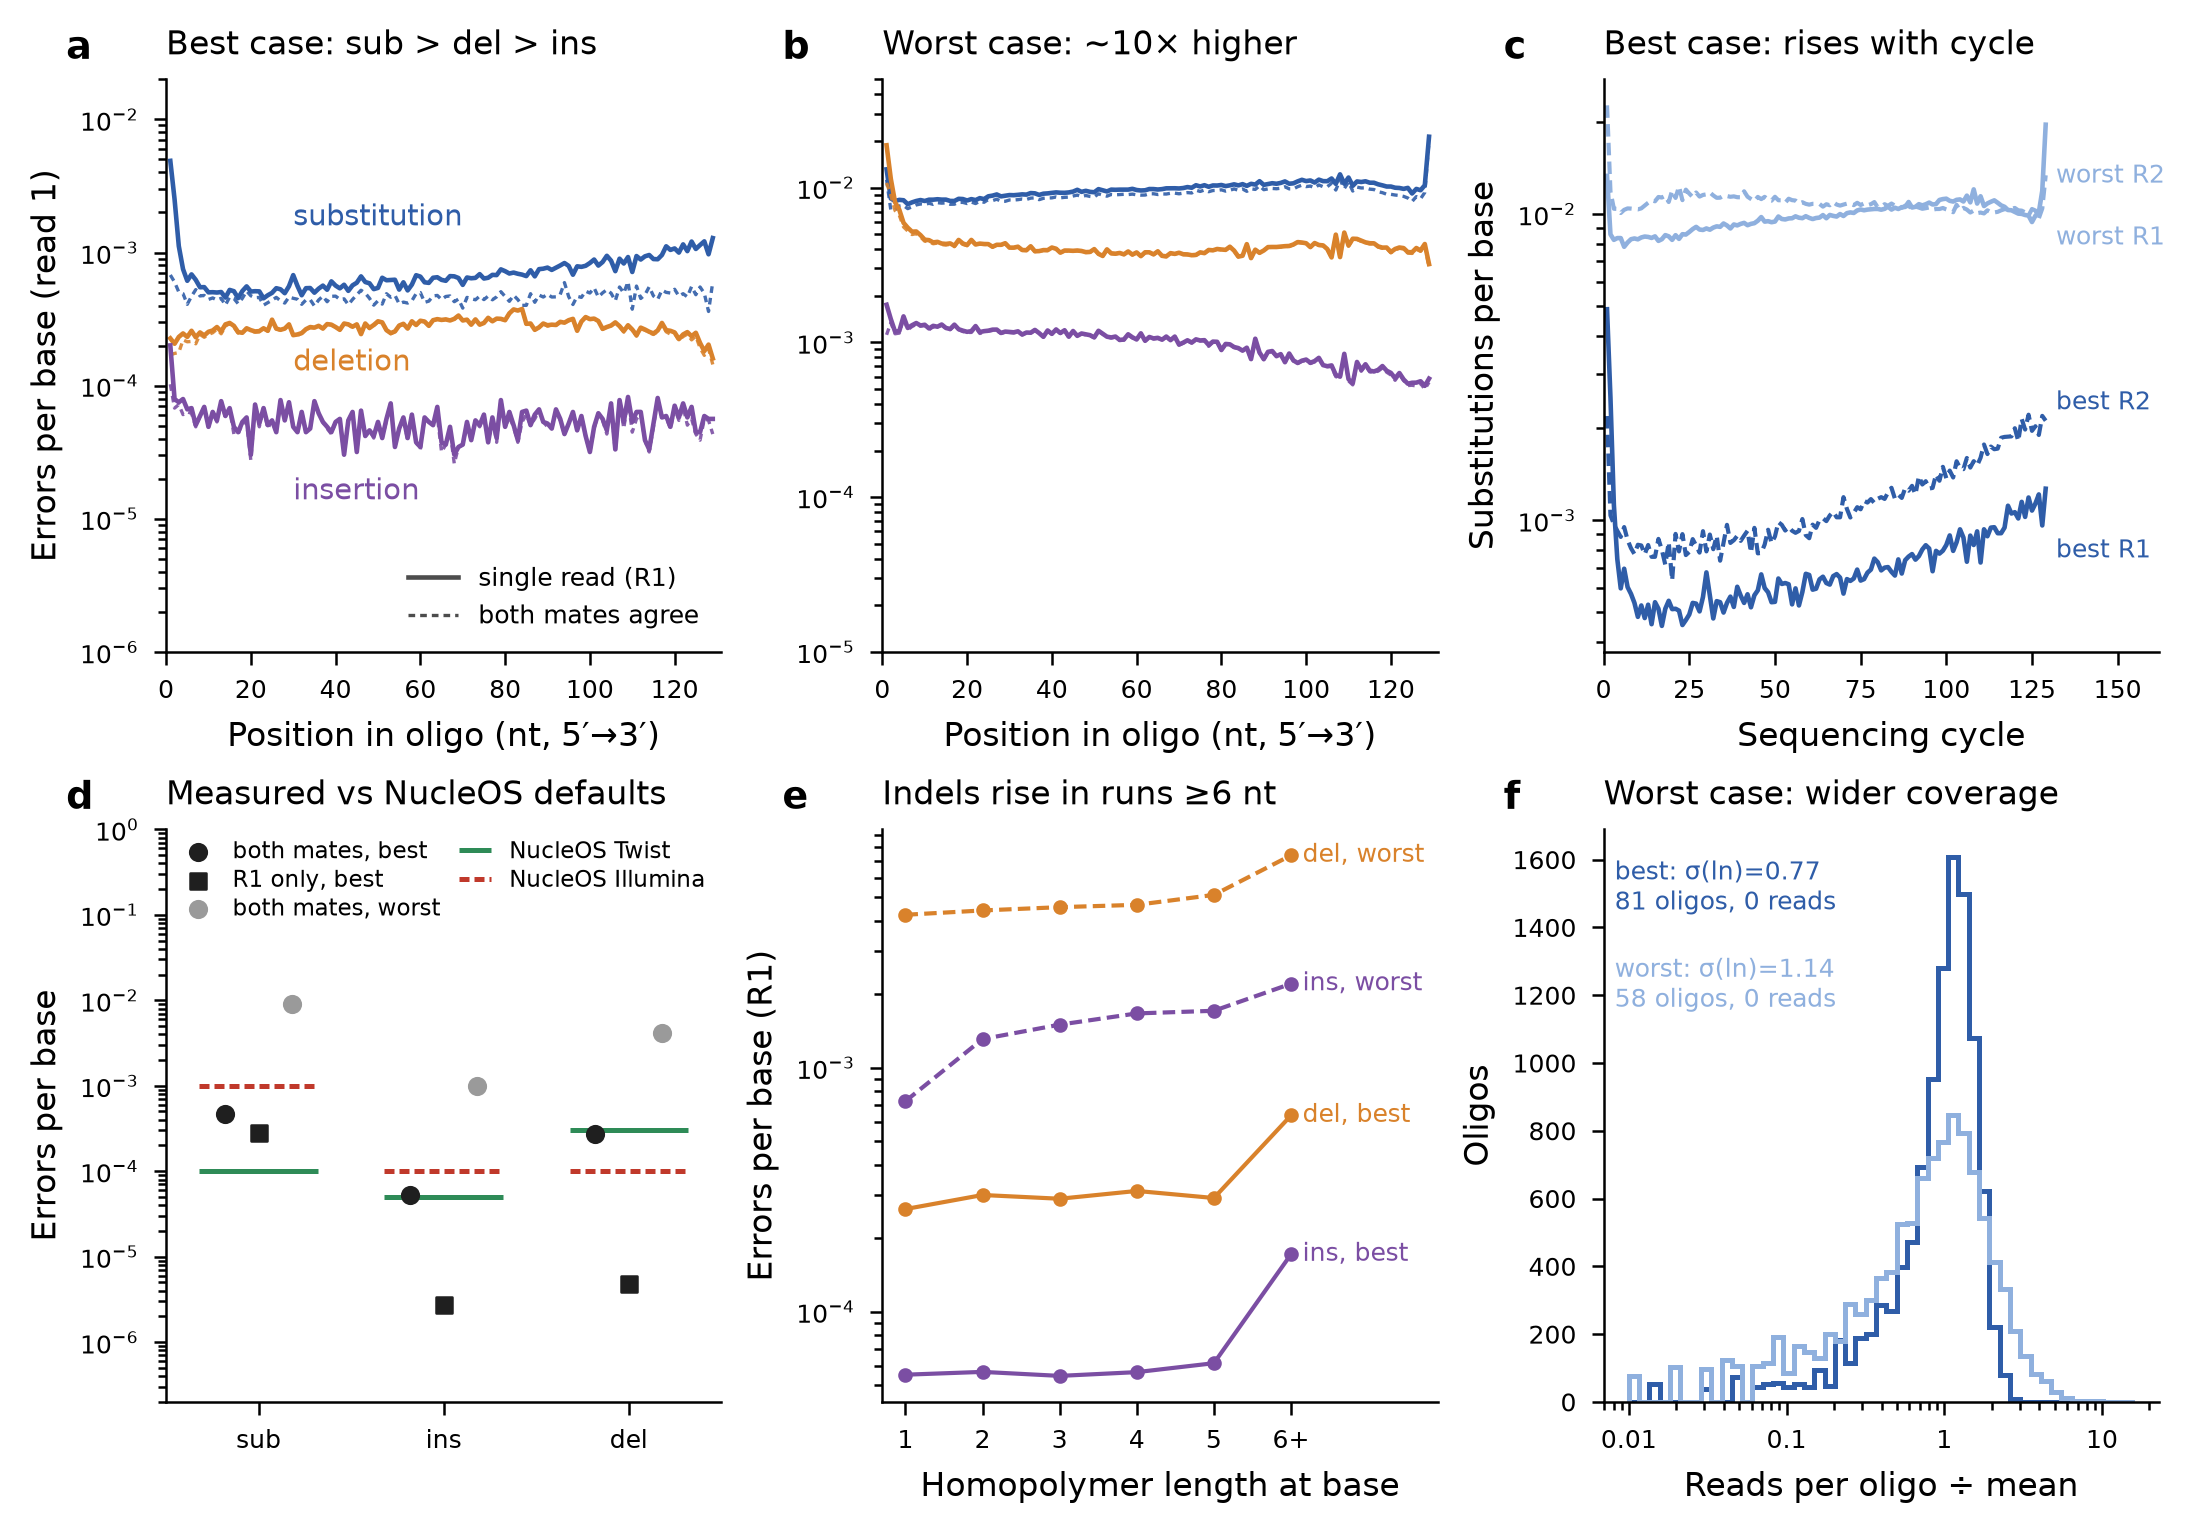
\includegraphics[width=\linewidth]{../docs/images/erp173549_error_profiles.png}
\caption{The two ERP173549 pools. (a, b) Read-1 error by position, single
read (solid) and both mates agreeing (dashed). (c) Substitutions by
sequencing cycle. (d) Molecule-level and sequencer rates against the
earlier defaults. (e) Indels by homopolymer length. (f) Reads per oligo
over the mean.}
\label{fig:channels}
\end{figure}

\section{Related work}
\label{sec:related}

\paragraph{Languages for designing DNA.} Cello compiles Verilog into
genetic circuits \cite{cello}, Eugene constrains how biological parts
compose \cite{eugene}, GSL describes genome edits \cite{gsl}, and SBOL is
a data standard for such designs \cite{sbol}. Their values are biological
parts; NucleScript's are stored files and pools read through noisy
machines. They meet at the strand: NucleScript's sequence literals are
checked for GC content, homopolymers and hairpins, as such tools also do.

\paragraph{Languages for laboratory work.} BioCoder writes protocols as
programs \cite{biocoder}. Puddle is an operating system and runtime for
digital microfluidics that corrects droplet errors as a program runs
\cite{puddle}. Puddle is the nearest relative in spirit, a full stack
over physical operations that can fail, and unlike NucleScript it drives
real hardware. NucleScript checks before anything runs instead: Puddle
handles failure dynamically and NucleScript plans for it statically.

\paragraph{DNA storage systems.} Bornholt et al.\ designed an archival
system with random access through PCR primers \cite{bornholt2016};
Organick et al.\ stored and randomly accessed about 200~MB
\cite{organick2018}; Takahashi et al.\ automated the whole cycle in one
device \cite{takahashi2019}. Chamaeleo \cite{chamaeleo}, MESA
\cite{mesa}, DNA-Storalator \cite{storalator} and the DNA Storage Toolkit
\cite{dnatoolkit} are libraries and simulators. NucleOS covers similar
ground; what they lack is a language over those parts with types and
effects a compiler checks. The systems papers ran real synthesis and
sequencing, which NucleOS has not.

\paragraph{Effects and physical quantities in types.} NucleScript's
effects follow the effect systems of Lucassen and Gifford
\cite{lucassen1988}: a function's effect is the join of its body's. Koka
carries effects in function types \cite{koka}, as NucleScript's ceilings
do. An error rate in a pool's type is closest to units of measure
\cite{kennedy1997}, a physical quantity the checker carries.

\paragraph{Testing and proving checkers.} The monitor and generator
follow QuickCheck \cite{quickcheck} and Csmith \cite{csmith}. The proof
is an induction over a big-step semantics with a semantic invariant on
closure values, mechanised in Lean \cite{lean4}. The method is standard;
what the proof adds is the rules it covers, in particular closures the
checker cannot trace and parameters without a ceiling, both of which the
implementation got wrong until the rules were written down.

\section{Limitations}
\label{sec:limits}

\begin{itemize}[leftmargin=*,itemsep=2pt]
\item \textbf{No wet-lab run.} No NucleScript program has driven a real
  synthesis or sequencing run. The order sheets have not been submitted.
  The real-read results use public datasets made by others.
\item \textbf{IDT's template.} IDT's oPools page takes Excel files only
  and, without an account, shows neither its template nor its column
  names, so NucleOS writes a CSV to paste into it. The length and pool
  size limits it checks matched the page on 8 November 2026.
\item \textbf{The proof covers a core.} See Section~\ref{sec:proof}; the
  fourth promise and the rest of the language rest on testing.
\item \textbf{Error-rate types are estimates.} The rates come from
  published profiles and from the measured channels of one study, and the
  consensus rule is a simple bound. They say nothing about a lab's own
  instruments.
\item \textbf{Synthesis and sequencing share a ceiling}, and
  \nsl{store} needs no confirmation, by design.
\item \textbf{The software has no DOI yet.} This report has one, but the
  repository's releases are not yet archived on Zenodo.
\end{itemize}

\section{Availability}

NucleOS and NucleScript are MIT-licensed at
\url{https://github.com/VyomKulshrestha/Nucle-OS}, and this report
describes release v0.1.70. A playground runs in the browser at
\url{https://nuclescript.github.io/playground/}. In the repository:

\begin{itemize}[leftmargin=*,itemsep=1pt]
\item \texttt{proofs/}: the Lean proof, built with \texttt{lake build} on
  Lean 4.35.0.
\item \texttt{nucle\_lang/tests/soundness.rs} and
  \texttt{soundness\_regressions.rs}: the monitor's tests and the eight
  regressions; \texttt{NSL\_SOUNDNESS\_PROGRAMS} sets the number of
  generated programs.
\item \texttt{scripts/erp173549/}: \texttt{prepare.py} rebuilds the
  Illumina pools and \texttt{decode.nsl} decodes them. The references are
  GPL-3.0, so no copy ships with the repository.
\end{itemize}

\begin{thebibliography}{99}
\small

\bibitem{allentoft2012}
M.~E. Allentoft, M.~Collins, D.~Harker, et al.
\newblock The half-life of DNA in bone: measuring decay kinetics in 158 dated fossils.
\newblock \emph{Proceedings of the Royal Society B}, 279(1748):4724--4733, 2012.
\newblock doi:10.1098/rspb.2012.1745.

\bibitem{biocoder}
V.~Ananthanarayanan and W.~Thies.
\newblock BioCoder: A programming language for standardizing and automating biology protocols.
\newblock \emph{Journal of Biological Engineering}, 4:13, 2010.
\newblock doi:10.1186/1754-1611-4-13.

\bibitem{eugene}
L.~Bilitchenko, A.~Liu, S.~Cheung, et al.
\newblock Eugene -- a domain specific language for specifying and constraining synthetic biological parts, devices, and systems.
\newblock \emph{PLoS ONE}, 6(4):e18882, 2011.
\newblock doi:10.1371/journal.pone.0018882.

\bibitem{bornholt2016}
J.~Bornholt, R.~Lopez, D.~M. Carmean, et al.
\newblock A DNA-based archival storage system.
\newblock In \emph{ASPLOS '16}, pages 637--649, 2016.
\newblock doi:10.1145/2872362.2872397.

\bibitem{storalator}
G.~Chaykin, O.~Sabary, N.~Furman, et al.
\newblock DNA-Storalator: a computational simulator for DNA data storage.
\newblock \emph{BMC Bioinformatics}, 26:204, 2025.
\newblock doi:10.1186/s12859-025-06222-0.

\bibitem{church2012}
G.~M. Church, Y.~Gao, and S.~Kosuri.
\newblock Next-generation digital information storage in DNA.
\newblock \emph{Science}, 337(6102):1628, 2012.
\newblock doi:10.1126/science.1226355.

\bibitem{quickcheck}
K.~Claessen and J.~Hughes.
\newblock QuickCheck: a lightweight tool for random testing of Haskell programs.
\newblock In \emph{ICFP '00}, pages 268--279, 2000.
\newblock doi:10.1145/351240.351266.

\bibitem{coudy2021}
D.~Coudy, M.~Colotte, A.~Luis, S.~Tuffet, and J.~Bonnet.
\newblock Long term conservation of DNA at ambient temperature. Implications for DNA data storage.
\newblock \emph{PLOS ONE}, 16(11):e0259868, 2021.
\newblock doi:10.1371/journal.pone.0259868.

\bibitem{lean4}
L.~de~Moura and S.~Ullrich.
\newblock The Lean 4 theorem prover and programming language.
\newblock In \emph{Automated Deduction -- CADE 28}, LNCS 12699, pages 625--635, 2021.
\newblock doi:10.1007/978-3-030-79876-5\_37.

\bibitem{erlich2017}
Y.~Erlich and D.~Zielinski.
\newblock DNA Fountain enables a robust and efficient storage architecture.
\newblock \emph{Science}, 355(6328):950--954, 2017.
\newblock doi:10.1126/science.aaj2038.

\bibitem{sbol}
M.~Galdzicki, K.~P. Clancy, E.~Oberortner, et al.
\newblock The Synthetic Biology Open Language (SBOL) provides a community standard for communicating designs in synthetic biology.
\newblock \emph{Nature Biotechnology}, 32(6):545--550, 2014.
\newblock doi:10.1038/nbt.2891.

\bibitem{gimpel2026}
A.~L. Gimpel, A.~Remschak, W.~J. Stark, R.~Heckel, and R.~N. Grass.
\newblock Comparison of state-of-the-art error-correction coding for sequence-based DNA data storage.
\newblock \emph{Nature Communications}, 2026.
\newblock doi:10.1038/s41467-026-70548-3. Reads: ENA study ERP173549.

\bibitem{goldman2013}
N.~Goldman, P.~Bertone, S.~Chen, et al.
\newblock Towards practical, high-capacity, low-maintenance information storage in synthesized DNA.
\newblock \emph{Nature}, 494(7435):77--80, 2013.
\newblock doi:10.1038/nature11875.

\bibitem{grass2015}
R.~N. Grass, R.~Heckel, M.~Puddu, D.~Paunescu, and W.~J. Stark.
\newblock Robust chemical preservation of digital information on DNA in silica with error-correcting codes.
\newblock \emph{Angewandte Chemie International Edition}, 54(8):2552--2555, 2015.
\newblock doi:10.1002/anie.201411378.

\bibitem{kennedy1997}
A.~J. Kennedy.
\newblock Relational parametricity and units of measure.
\newblock In \emph{POPL '97}, pages 442--455, 1997.
\newblock doi:10.1145/263699.263761.

\bibitem{koka}
D.~Leijen.
\newblock Koka: Programming with row polymorphic effect types.
\newblock \emph{EPTCS}, 153:100--126, 2014.
\newblock doi:10.4204/EPTCS.153.8.

\bibitem{lucassen1988}
J.~M. Lucassen and D.~K. Gifford.
\newblock Polymorphic effect systems.
\newblock In \emph{POPL '88}, pages 47--57, 1988.
\newblock doi:10.1145/73560.73564.

\bibitem{cello}
A.~A.~K. Nielsen, B.~S. Der, J.~Shin, et al.
\newblock Genetic circuit design automation.
\newblock \emph{Science}, 352(6281):aac7341, 2016.
\newblock doi:10.1126/science.aac7341.

\bibitem{organick2018}
L.~Organick, S.~D. Ang, Y.-J. Chen, et al.
\newblock Random access in large-scale DNA data storage.
\newblock \emph{Nature Biotechnology}, 36(3):242--248, 2018.
\newblock doi:10.1038/nbt.4079.

\bibitem{yinyang}
Z.~Ping, S.~Chen, G.~Zhou, et al.
\newblock Towards practical and robust DNA-based data archiving using the yin--yang codec system.
\newblock \emph{Nature Computational Science}, 2:234--242, 2022.
\newblock doi:10.1038/s43588-022-00231-2.

\bibitem{chamaeleo}
Z.~Ping, H.~Zhang, S.~Chen, et al.
\newblock Chamaeleo: a robust library for DNA storage coding schemes.
\newblock \emph{bioRxiv}, 2020.
\newblock doi:10.1101/2020.01.02.892588.

\bibitem{hedges}
W.~H. Press, J.~A. Hawkins, S.~K. Jones, J.~M. Schaub, and I.~J. Finkelstein.
\newblock HEDGES error-correcting code for DNA storage corrects indels and allows sequence constraints.
\newblock \emph{PNAS}, 117(31):18489--18496, 2020.
\newblock doi:10.1073/pnas.2004821117.

\bibitem{rashtchian2017}
C.~Rashtchian, K.~Makarychev, M.~R\'acz, et al.
\newblock Clustering billions of reads for DNA data storage.
\newblock In \emph{Advances in Neural Information Processing Systems 30 (NeurIPS 2017)}, 2017.

\bibitem{mesa}
M.~Schwarz, M.~Welzel, T.~Kabdullayeva, et al.
\newblock MESA: automated assessment of synthetic DNA fragments and simulation of DNA synthesis, storage, sequencing and PCR errors.
\newblock \emph{Bioinformatics}, 36(11):3322--3326, 2020.
\newblock doi:10.1093/bioinformatics/btaa140.

\bibitem{dnatoolkit}
P.~Sharma, G.~G. Yipeng, B.~Gao, et al.
\newblock DNA Storage Toolkit: A modular end-to-end DNA data storage codec and simulator.
\newblock In \emph{ISPASS 2024}, pages 144--155, 2024.
\newblock doi:10.1109/ISPASS61541.2024.00023.

\bibitem{trellisbma}
S.~R. Srinivasavaradhan, S.~Gopi, H.~D. Pfister, and S.~Yekhanin.
\newblock Trellis BMA: Coded trace reconstruction on IDS channels for DNA storage.
\newblock In \emph{IEEE International Symposium on Information Theory (ISIT)}, pages 2453--2458, 2021.
\newblock doi:10.1109/ISIT45174.2021.9517821.

\bibitem{takahashi2019}
C.~N. Takahashi, B.~H. Nguyen, K.~Strauss, and L.~Ceze.
\newblock Demonstration of end-to-end automation of DNA data storage.
\newblock \emph{Scientific Reports}, 9:4998, 2019.
\newblock doi:10.1038/s41598-019-41228-8.

\bibitem{puddle}
M.~Willsey, A.~P. Stephenson, C.~Takahashi, et al.
\newblock Puddle: A dynamic, error-correcting, full-stack microfluidics platform.
\newblock In \emph{ASPLOS '19}, pages 183--197, 2019.
\newblock doi:10.1145/3297858.3304027.

\bibitem{gsl}
E.~H. Wilson, S.~Sagawa, J.~W. Weis, et al.
\newblock Genotype Specification Language.
\newblock \emph{ACS Synthetic Biology}, 5(6):471--478, 2016.
\newblock doi:10.1021/acssynbio.5b00194.

\bibitem{csmith}
X.~Yang, Y.~Chen, E.~Eide, and J.~Regehr.
\newblock Finding and understanding bugs in C compilers.
\newblock In \emph{PLDI '11}, pages 283--294, 2011.
\newblock doi:10.1145/1993498.1993532.

\end{thebibliography}

\end{document}
